\documentclass{amsart}
\usepackage{amsmath,amsfonts,amssymb}
\usepackage{mathrsfs}
\usepackage{graphicx}
\usepackage{caption}
\usepackage{float}
\usepackage{subfig}
\usepackage[romanian]{babel}
\usepackage[colorlinks,unicode]{hyperref}
\usepackage[foot]{amsaddr}
\usepackage{wallpaper}
\usepackage{listings}
\usepackage{color}


%\numberwithin{equation}{section}

%\renewcommand{\emailaddrname}{\itshape Adresa e-mail}

\definecolor{mygreen}{rgb}{0,0.6,1}
\definecolor{mygray}{rgb}{0.5,0.5,0.5}
\definecolor{mymauve}{rgb}{0.58,0,0.82}

\lstset{ %
  backgroundcolor=\color{white},   % choose the background color
  basicstyle=\footnotesize,        % size of fonts used for the code
  breaklines=true,                 % automatic line breaking only at whitespace
  captionpos=b,                    % sets the caption-position to bottom
  commentstyle=\color{mygreen},    % comment style
  escapeinside={\%*}{*)},          % if you want to add LaTeX within your code
  keywordstyle=\color{blue},       % keyword style
  stringstyle=\color{mymauve},     % string literal style
}


\makeatletter
\def\@setemails{%
  \ifnum\theg@author > 1
    \mbox{{\itshape Adrese e-mail}:\space}{\ttfamily\emails}.
  \else
    \mbox{{\itshape Adresa e-mail}:\space}{\ttfamily\emails}.
  \fi%
}
\makeatother

\addtolength{\wpXoffset}{-5.38cm}
\addtolength{\wpYoffset}{11.5cm}
\CenterWallPaper{0.15}{FMI.png}


\title{Medii de Proiectare și Programare}

\author{Madaras Andrei Iulian}
%\author{Author 2}
\address{Facultatea de Matematic\u{a} \c{s}i Informatic\u{a} , Anul 3, Sec\c{t}ia Informatic\u{a} Aplicat\u{a}}
%aici se va completa adresa e-mail
\email{andrei.madaras01@e-uvt.ro}


\begin{document}


\maketitle

\section{Enunțul temei/proiectului}

Aici se vor specifica cerințele temei/proiectului ...

Aceasta este o list\u{a} numerotat\u{a}:
\begin{itemize}
\item[(1)] primul element;
\item[(2)] al doilea element;
\item[(3)] al treilea element.
\end{itemize}

\section{Rezolvarea problemei}

Enumerarea pașilor parcurși pentru crearea scheletului aplicației Windows standard.

Soluționarea temei presupune parcurgerea a două etape:

\subsection{Proiectarea interfeței aplicației}

Se specifică tipul controalelor introduse în cadrul resursei dialog a aplicației, precum și toate setările realizate pentru acestea. 

Se indică, dacă este cazul, variabilele utilizate în cadrul proiectului, precizând toate detaliile despre acestea (căror controale le-au fost asociate, caterogia, tipul, numele, clasa din care fac parte, dacă au fost inițializate etc.

\subsection{Asigurarea funcționalității aplicației}

Se descriu pașii pentru asocierea unei funcții pentru un control, specificând tipul mesajului interceptat, clasa din care face parte, numele etc.

\texttt{Codul funcției (\^{i}n VisualC++)}

Secven\c{t}a de cod corespunz\u{a}toare ...

\begin{lstlisting}[language=C++]{Name=test2}
void CEuclidDlg::OnBnClickedCalculeaza()
{
	// TODO: Add your control notification handler code here 
	UpdateData(); 
	int x,y,r;
	x=A;
           y=B;
	if(x==y && y==0)
	{
	 AfxMessageBox((LPCWSTR)L"A si B nu pot fi simultan nule!");
	 return;
	}
    if(y!=0)
		do
		{
		   r=x%y;
	        	   x=y;
	       	   y=r;
		}
		while(r!=0);
		cmMdc=x;
		cmmmc=A*B/cmMdc;
		UpdateData(FALSE);
 \end{lstlisting}

Interfața aplicației, după afișarea rezultatelor, se poate observa \^{i}n figura \ref{fig1}.

\begin{figure}[ht]
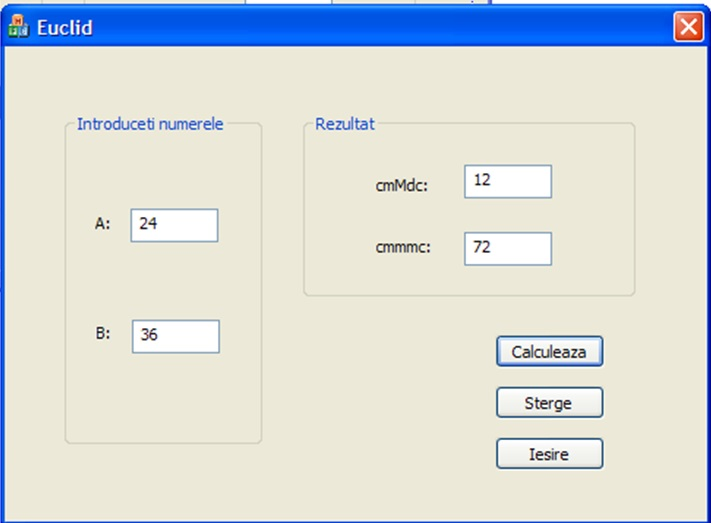
\includegraphics[width=12cm]{Interfata.jpg}
\caption{Interfața aplicației}
\label{fig1}
\end{figure}
 

Aceasta este o ecua\c{t}ie (formul\u{a}) numerotat\u{a}:
\begin{equation}\label{pitagora}
a^2+b^2=c^2.
\end{equation}

\section{Concluzii}

Rezultatele acestei sec\c{t}iuni se g\u{a}sesc \^{\i}n \cite{Aut}.


Aceasta este o list\u{a} nenumerotat\u{a}:
\begin{itemize}
\item primul element;
\item al doilea element;
\item al treilea element.
\end{itemize}

A\c{s}a se includ două figuri alăturate:
        
\begin{figure}[ht]
\begin{tabular}{cc}
\subfloat[Interfața proiectată]{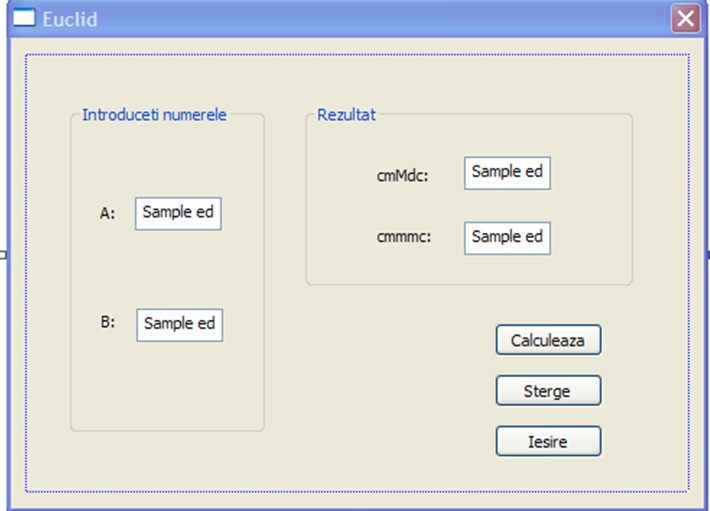
\includegraphics[width=6cm]{Interfata0.jpg}} &
\subfloat[... și după execuție]{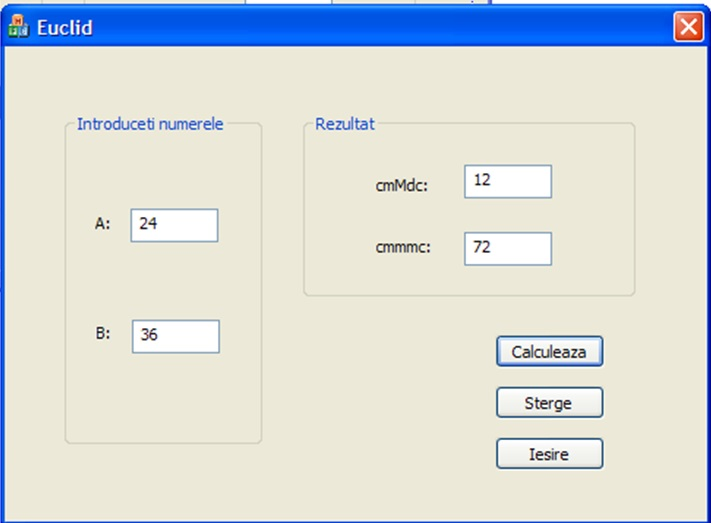
\includegraphics[width=5.9cm]{Interfata.jpg}}
\end{tabular}
\caption{Interfața aplicației}
\end{figure}

% lucrarile incluse in bibliografie se citeaza obligatoriu in textul lucrarii
% folosind comanda \cite
\begin{thebibliography}{99}
\bibitem{N1N2} \textsc{P1. Nume1} \c{s}i \textsc{P2. Nume2}, \emph{Titlu carte}, Numele editurii, Localitatea, Anul apar\c{t}iei.
\bibitem{Aut} \textsc{P. Autor}, Titlu lucrare, \emph{Numele revistei} \textbf{num\u{a}r} (anul apari\c{t}iei), pag. \^{\i}nceput--pag. sf\^ar\c{s}it.
\bibitem{link1} \url{https://ro.wikibooks.org/wiki/LaTeX_(carte)/Gestiunea_bibliografiei}
\end{thebibliography}
\end{document}